%%%%%%%%%%%%%%%%%%%%%%%%%%%%%%%
%%%%%%%%%%%%%%%%%%%%%%%%%%%%%%%
\chapter{Results\label{ch:results}}
%%%%%%%%%%%%%%%%%%%%%%%%%%%%%%%
This chapter presents a summary of the appended papers, including research activities
and a selection of the important results, and highlights the main achievements. A model for the roll motion is developed in Paper \ref{pap:rolldamping}. A manoeuvring model is developed in Paper \ref{pap:daiyong} and Paper \ref{pap:pit} and the model generalization is addressed in Paper \ref{pap:pit}.

\section{Summary of Paper \ref{pap:rolldamping}}
\subsection*{"\nameref{pap:rolldamping}"}
System identification of ship roll motion, including roll damping and stiffness, is developed in in Paper \ref{pap:rolldamping}. In the second generation of intact stability criteria, the IMO addressed the importance of ships having sufficient roll damping to avoid large roll motions, parametric rolling, and excessive acceleration \parencite{imo_finalization_2016}. These phenomena have been well known for a very long time. Parametric roll was observed already by \parencite{froude_rolling_1861} and has been on the agenda of the marine research community since the early 1950s \parencite{galeazzi_early_2013}; it has received much more attention since \parencite{france_investigation_2001} showed that the APL China casualty in 1998, where a post-Panamax C11 class container ship lost almost a third of its containers, was most likely caused by head sea parametric rolling. The damping of roll motion plays an important part during the above-mentioned phenomena. It has been shown that the relatively small difference in the roll damping prediction they obtained with small method variation, could mean the difference between severe roll angles and hardly noticeable motions \parencite{soder_ikeda_2019}.

The objective in Paper \ref{pap:rolldamping} was therefore to improve the roll damping predictions for modern ships. The roll damping was studied using time series data from 250 (see Fig. \ref{fig:ship_types}) roll decay tests (see \autoref{sec:roll}) assembled from the Maritime Dynamics Laboratory at SSPA Sweden AB (\href{www.sspa.se}{www.sspa.se}).

\begin{figure}[H]
    \centering
    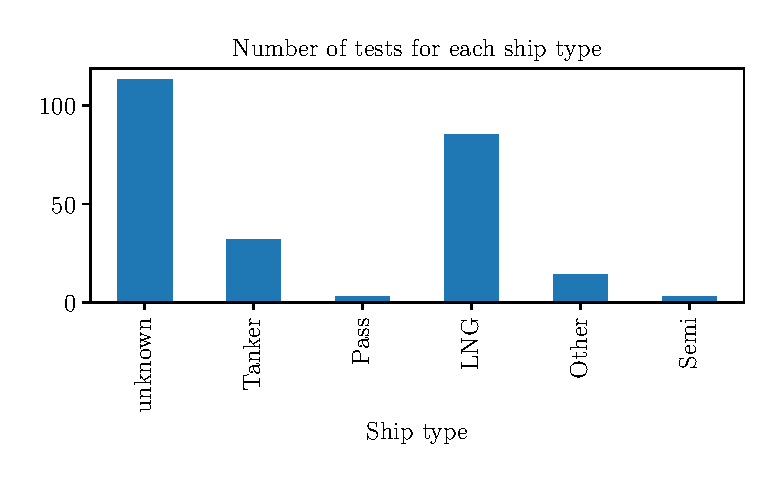
\includegraphics[width=0.5\columnwidth]{kappa/images/ship_types.eps}
    \caption{Number of tests per ship type}
    \label{fig:ship_types}
\end{figure}

\noindent The work was broken down to the following subtasks: 
\begin{itemize}
    \item Find the mathematical model that best describes the roll motion
    \item Identify the parameters in this model for all the tests
    \item Compare the identified parameters with state of art prediction
    \item Develop a generic roll damping model for all ships, using the identified parameters
    \begin{itemize}
        \item Grey-box model
        \item Black-box model
    \end{itemize}
\end{itemize}

\noindent The work is also summarized in \autoref{fig:paper1_overview}. System identification on the time series from the roll decay database was performed with the linear (\autoref{eq:roll_decay_equation_himeno_linear}), quadratic (\autoref{eq:roll_decay_equation_himeno_quadratic_b}) and cubic model (\autoref{eq:roll_decay_equation_cubic}). Roll damping parameters identified from the model that was found to be the best was used to build a roll damping database. The identified roll dampings could then be compared with corresponding predictions with the Simplified-Ikedas method \cite{kawahara_simple_2011}, being the state of art prediction for ship roll damping.
The generic roll damping model was then developed as a grey-box model or a pure black-box model.
\begin{figure}[H]
    \centering
    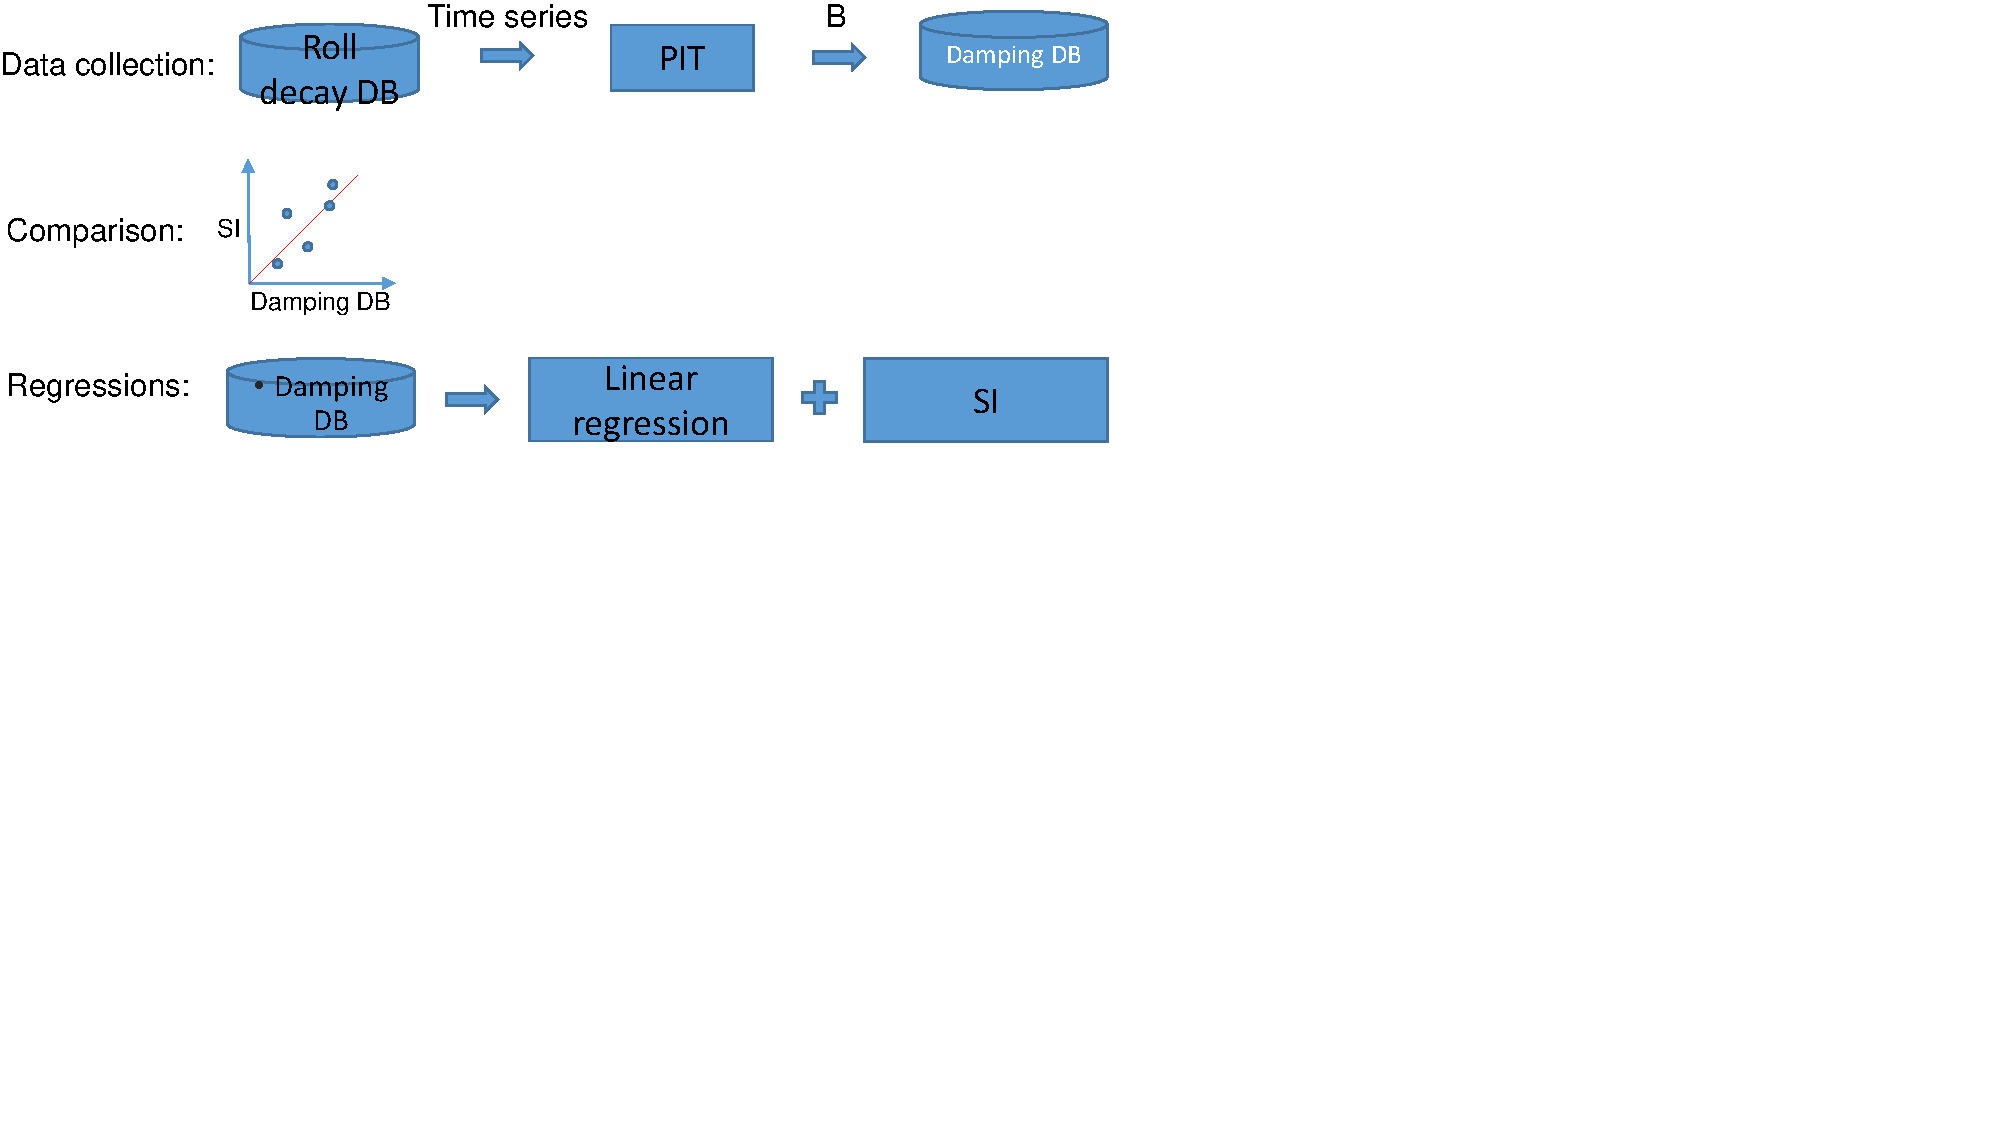
\includegraphics[width=\linewidth]{kappa/images/workflow.pdf}
    \caption{Overview of the work conducted for Paper \ref{pap:rolldamping}}
    \label{fig:paper1_overview}
\end{figure}

\subsection{Best mathematical model for the roll motion}
System identification on the linear, quadratic and cubic model was conducted using both the ''integration approach'' (described in \autoref{sec:integration_approach}) and the ''derivation approach'' (described in \autoref{sec:derivation_approach}).
Results from simulations with the identified models is shown for one of the roll-decay tests in \autoref{fig:roll_decay_compare}. It can be seen that the cubic and quadratic model reproduce the model test well and that the the linear model is too simple to have a good representation for both smaller and larger roll angles. The amplitude decrement $\phi_a$ and roll damping $B$ for each oscillation can also be visualized as seen in \autoref{fig:roll_decay}.

\begin{figure}[!htb]
    \centering
    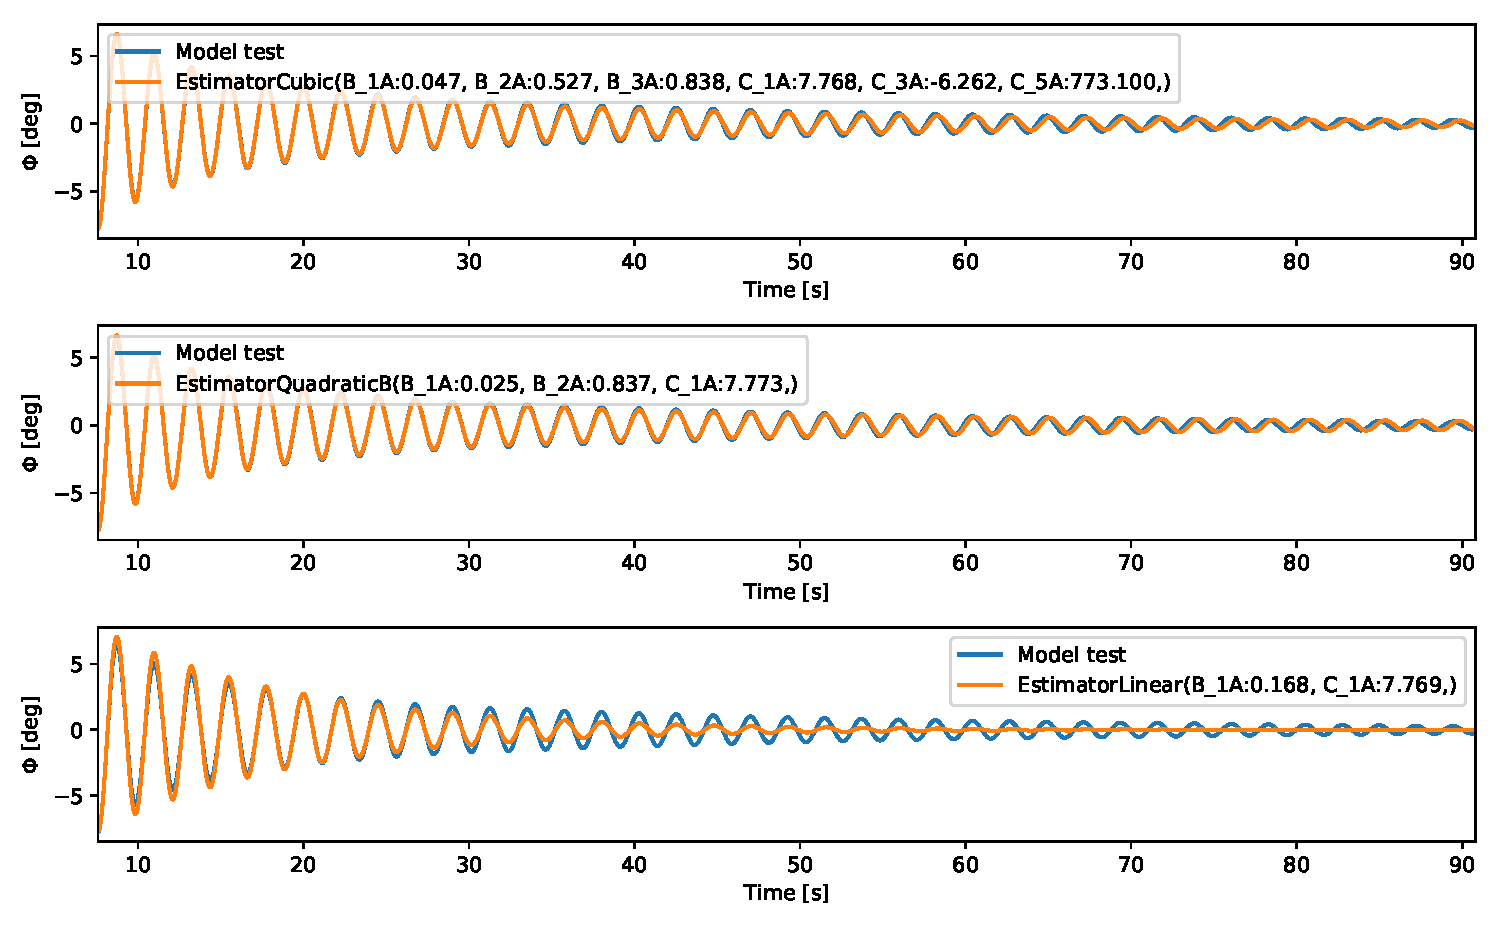
\includegraphics[width=\linewidth]{kappa/images/roll_decay_model_compare.pdf}
    \caption{Roll decay estimation with identified cubic, quadratic and linear model.}
    \label{fig:roll_decay_compare}
\end{figure}

\begin{figure}[!htb]
    \begin{subfigure}[b]{0.45\textwidth}
        \centering
        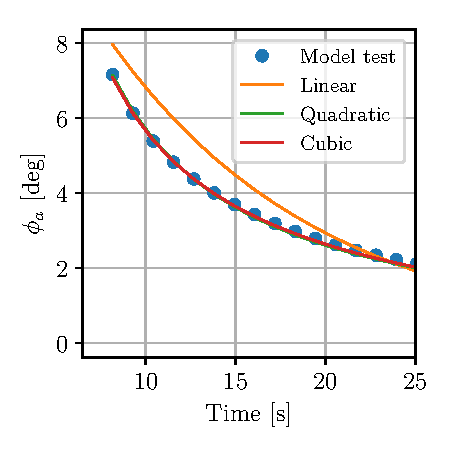
\includegraphics[]{kappa/images/roll_decay_amplitude.pdf}
        \caption{Amplitude decrements}
        \label{fig:roll_decay_amplitude}
    \end{subfigure}
        ~ %add desired spacing between images, e. g. ~, \quad, \qquad, \hfill etc. 
      %(or a blank line to force the subfigure onto a new line)
    \begin{subfigure}[b]{0.45\textwidth}
        \centering
        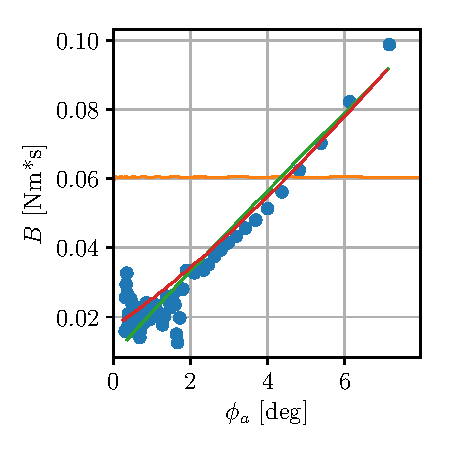
\includegraphics[]{kappa/images//roll_decay_damping.pdf}
        \caption{Dampings}
        \label{fig:roll_decay_damping}
    \end{subfigure}
    \caption{Roll decay model test, linear-, quadratic- and cubic-model}
    \label{fig:roll_decay}
\end{figure}

\noindent The best parameter estimations were obtained using the ''integration approach''.
The goodness of fit of the linear, quadratic and cubic model are described using the coefficient of determination:
\begin{equation} \label{eq:R2}
%R^2=1-\frac{SS_{res}}{SS_{tot}}
R^2=1-\frac{\sum\limit_{i=1}^{n}(\phi_{i}-\hat{\phi}_i)^2}{\sum\limit_{i=1}^{n}(\phi_i-\bar \phi)^2}
\end{equation}
where $\phi_i$ is the model test roll angle at time step $i$, $\bar \phi$ is the mean roll angle from the model test and $\hat{\phi}_i$ is the predicted roll angle (with linear, quadratic or cubic model). The average goodness of fit $R^2$ was 0.995 for the cubic model, 0.993 for the quadratic, and 0.986 for the linear model. This means that the quadratic model is almost as good as the cubic model in describing the roll motion. The quadratic model with fewer parameters than the cubic model is expected to have a better generalization at the same accuracy and is therefore selected as the best mathematical model for the roll motion. 

\subsection{Compare with state of art prediction}
Ikeda's method divides roll damping into five damping components: the friction component $B_F$, the eddy component $B_E$, the lift component $B_L$, the wave component $B_W$ and the bilge keel component $B_{BK}$, as in the following Eq.(\ref{eq:ikeda}), 
\begin{equation} \label{eq:ikeda}
B_{44} = B_F + B_E + B_L + B_W + B_{BK}
\end{equation}
where the wave and eddy components require strip-theory based hydrodynamic analysis to obtain the ship's shape coefficients. The hydrodynamic analysis requires the ship's exact hull geometries. It might be time consuming to build the geometry model and perform the strip-theory based hydrodynamic analysis. Sometimes, a ship's hull geometry is simply not available for such purposes. 

A simplified Ikeda method (SI-method) was proposed by \parencite{kawahara_simple_2011} is used in Paper \ref{pap:rolldamping} to calculate all the damping components including the eddy component $B_E$ and wave component $B_W$. The semi-empirical formulas describe four of the five roll damping components at motion frequency $\omega$ for a given roll amplitude $\phi_a$ at zero ship speed. A speed dependency was introduced by adding a fifth damping term $B_L$ and a speed correction to $B_W$ and $B_E$ as described in \parencite{ikeda_velocity_1979}, giving a function: 
\begin{equation} \label{eq:simplified_ikeda_equation}
\left( B_{F}, \  B_{W}, \  B_{E}, \  B_{BK}, \  B_{L}\right) = \operatorname{f}\left(L_{pp},beam,C_{b},A_{0},OG,\phi_{a},BK_{L},BK_{B},\omega,T,V\right)
\end{equation}


\noindent The formulas within $f$ can be referred to \parencite{ikeda_velocity_1979, kawahara_simple_2011} with the implementation in \cite{alexandersson_martinlarsalbertrolldecay-estimators_2020}.
It should be noted that this method may be only efficiently used to estimate the roll damping of ships within the boundaries \parencite{kawahara_simple_2011}:
\begin{equation}
    \label{eq:SI_limits}
     \left\{
     \begin{array}{ll}
    0.5 \leq C_b \leq 0.85,\hspace{0.5cm} 
    0 \leq \hat{\omega} \leq 1.0,
    \hspace{0.5cm}
    0.9 \leq A_0 \leq 0.99,\\
    2.5\leq Beam/T \leq 4.5, \hspace{1cm}
    0.01 \leq BK_B/Beam \leq 0.06, \\
        -1.5 \leq OG/T \leq 0.2,
     \hspace{1cm}
    0.05 \leq BK_L/L_{PP} \leq 0.4.
    \end{array}
    \right.
\end{equation}

\noindent The total roll damping is predicted as the sum (\autoref{eq:ikeda}) of the damping contributions (\autoref{eq:simplified_ikeda_equation}). This damping can be compared with the linearized equivalent damping $B_e$, calculated for a certain roll angle $\phi_a$ with the identified roll damping parameters $B_1$ and $B_2$ \cite{himeno_prediction_1981},
\begin{equation} \label{eq:B_e_equation}
B_{e} = B_{1} + \frac{8 B_{2} \omega_{0} \phi_{a}}{3 \pi}
\end{equation}


\noindent The $B_e$ coefficient can be made non-dimensional according to \parencite{himeno_prediction_1981}, giving the non-dimensional equivalent linear damping coefficient $\hat{B_e}$. This one is more convenient to use when comparing roll damping for different ships,
\begin{equation} \label{eq:be_eqvalent}
    \hat{B_e} = \frac{B_e}{\rho \bigtriangledown Beam^2} \sqrt{\frac{Beam}{2g}},
\end{equation}
\noindent where $\rho$, $\bigtriangledown$ and $Beam$ stand for fluid density, displacement volume, and breadth of a ship, respectively. Prediction error plots of $\hat{B_e}$ from the Simplified Ikeda and identified damping from the model tests are shown in \autoref{fig:si_model_within}. A comparison of predictions with roll amplitudes in the range 0 to 10 degrees are shown for all ships (no limits) and for only ships within the limits of the method (\autoref{eq:SI_limits}). The $R^2$ values of the predictions are shown in \autoref{tab:si_validation}. There is reasonable agreement between the predicted roll damping and model tests for ships withing the limits. There is however a very poor agreement for ships outside the limits. It can also be noted that most of the points are outside the limits of the method.

\begin{figure}[!htb]
    \centering
    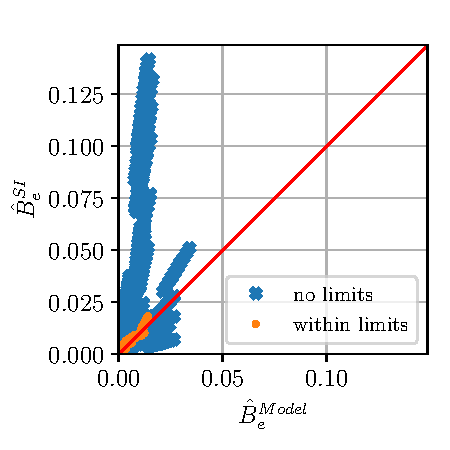
\includegraphics[width=0.75\textwidth]{kappa/images/si_model_within.pdf}
    \vspace{-0.5cm}
    \caption{Prediction error plot of the Simplified Ikedas method within and outside its limits}
    \label{fig:si_model_within}
\end{figure}


\begin{table}[H]
    \centering
    \caption{Validation of SI within and outside limits}
   \begin{tabular}{lrr}
\toprule
{} &  $R^2$ &  Number of points \\
\midrule
SI no limits     & -46.35 &              1470 \\
SI within limits &   0.83 &               120 \\
\bottomrule
\end{tabular}

    \label{tab:si_validation}
\end{table}
    

\noindent The largest contribution to the error in the predictions comes from the wave damping $B_W$ as seen in \autoref{fig:component_residual}
\begin{figure}[!htb]
    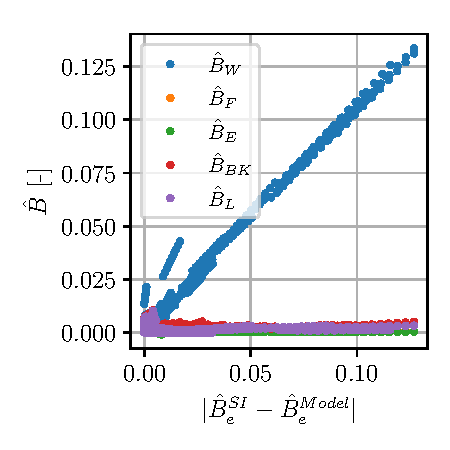
\includegraphics[width=0.75\textwidth]{kappa/images/component_residual.pdf}
    \caption{Residuals vs. components}
    \label{fig:component_residual}
\end{figure}
A Comparison of the Simplified-Ikedas method and the original Ikeda's method was also carriet out in Paper \ref{pap:rolldamping}, to see whether the observed deviations are result from extrapolation or inherent in the original method. In Ikeda's method, more detailed information about the ship hull geometry is needed so that $B_W$ can be calculated with a strip method and $B_E$ can be calculated using sectional Lewis coefficients. It was possible to collect the required hull inputs for 15 ships in the database. These ships were used in 50 of the reference roll decay tests: all but one of the tests exceed the limits. Ikeda's method has a much better agreement for these exceeding model tests according to Fig.\ref{fig:si_ikeda_model} and the calculated $R^2$ in Table \ref{tab:si_ikeda_validation}.

\begin{figure}[!htb]

    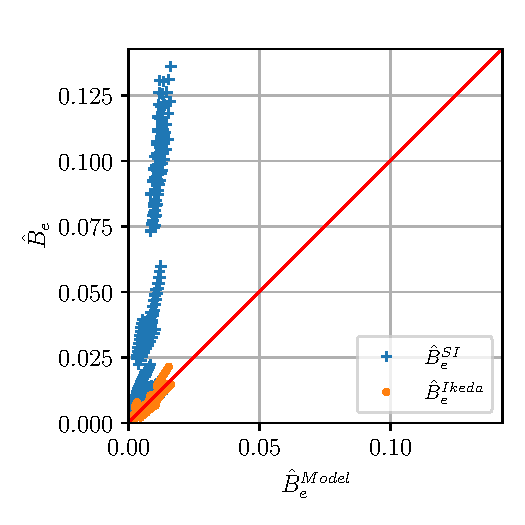
\includegraphics[width=0.75\textwidth]{kappa/images/si_ikeda_model.pdf}
    \caption{Comparison of SI, Ikeda and model tests}
    \label{fig:si_ikeda_model}

\end{figure}


\begin{table}[H]
    \centering
    \caption{Validation of SI and Ikeda.}
   \begin{tabular}{lrr}
\toprule
{} &   $R^2$ &  Number of points \\
\midrule
Ikeda        &    0.84 &               500 \\
SI no limits & -127.95 &               500 \\
\bottomrule
\end{tabular}

    \label{tab:si_ikeda_validation}
\end{table}
    



\subsection{Generic roll damping model}
\label{sec:genericrolldampingmodel}
A serial grey-box model for ship roll damping (see Fig.\ref{fig:greyrolldamping}) is also developed in Paper \ref{pap:rolldamping}. 
This is expanding the system identification, not only focusing on one ship, but rather all modern ships. 
Simplified Ikeda's method \cite{kawahara_simple_2011} is used as the white box model, which is combined with a following black-box correction model.

\begin{figure}[!htb]
    
    \centering
    \begin{tikzpicture}[node distance=2cm]
    \node (white-box) [white-box] {Simplified Ikeda};
    \node (B_BK) [io, right of=white-box, xshift=0.90cm, yshift=1.5cm] {$\hat{B_{BK}}$};
    \node (B_E) [io, right of=white-box, xshift=0.75cm, yshift=0.75cm] {$\hat{B_{E}}$};
    \node (B_F) [io, right of=white-box, xshift=0.75cm, yshift=0cm] {$\hat{B_{F}}$};
    \node (B_L) [io, right of=white-box, xshift=0.75cm, yshift=-0.75cm] {$\hat{B_{L}}$};
    \node (B_W) [io, right of=white-box, xshift=0.75cm, yshift=-1.5cm] {$\hat{B_{W}}$};
    
    
    \node (black-box) [black-box, right of=B_F, xshift=0.75cm] {Black-box};
    \draw [arrow] (white-box) -- (B_BK);
    \draw [arrow] (white-box) -- (B_E);
    \draw [arrow] (white-box) -- (B_F);
    \draw [arrow] (white-box) -- (B_L);
    \draw [arrow] (white-box) -- (B_W);
    
    \draw [arrow] (B_BK) -- (black-box);
    \draw [arrow] (B_E)  -- (black-box);
    \draw [arrow] (B_F)  -- (black-box);
    \draw [arrow] (B_L)  -- (black-box);
    \draw [arrow] (B_W)  -- (black-box);
    
    
    \node (B) [io, right of=black-box, xshift=0.75cm, yshift=0cm] {$B$};
    \draw [arrow] (black-box)  -- (B);
    
    \end{tikzpicture}
    \caption{Grey-box model to predict roll damping}
    \label{fig:greyrolldamping}
\end{figure}

\noindent The roll damping data set, obtained from the roll motion investigation, is used to train the black-box part of the grey-box model. The black-box correction model of the output components from the Simplified Ikeda's method are shown in (Eq.\ref{eq:polynom_correction}),
\begin{equation} \label{eq:polynom_correction}
\hat{B_{e}} = 1.106 \hat{B_{BK}} - 0.9124 \hat{B_{E}} + 4.282 \hat{B_{F}} + 0.7457 \hat{B_{L}} + 0.1844 \hat{B_{W}} + 0.004999 \phi_{a} - 0.0005097
\end{equation}


\noindent Large corrections of the skin friction damping $\hat{B_F}$ and wave damping $\hat{B_W}$ are suggested by this expression. This is because the Simplified Ikeda's method is not very accurate for this dataset, where most of the ships in the dataset exceed the limits of the method. A pure black-box model is also devloped in Paper \ref{pap:rolldamping} (see Eq.\ref{eq:polynom_complex}),
\begin{equation} \label{eq:polynom_complex}
\begin{aligned} 
 \hat{B_{e}} = - 0.02578 A_{0} V - 0.02705 BK_{B} V + \\ 
 0.008993 BK_{L} V - 0.03191 C_{b} V - 0.2028 OG V + \\ 
 0.003472 V^{2} + \\ 
 0.004234 V \hat{\omega_{0}} - 0.002591 V \phi_{a} - 0.008384 V beam + \\ 
 0.05048 V + \\ 
 0.007814 \hat{\omega_{0}}^{2} + \\ 
 0.03882 \hat{\omega_{0}} \phi_{a} - 0.001069 \\ 
 \end{aligned}
\end{equation}


\noindent where non-dimensional frequency $\hat{\omega_0}$ is calculated with \autoref{eq:omega0_hat_equation} \cite{himeno_prediction_1981},
\begin{equation} \label{eq:omega0_hat_equation}
\omega_{hat} = \frac{\sqrt{2} \omega_{0} \sqrt{\frac{beam}{g}}}{2}
\end{equation}


\noindent When constructing a regression model from a data set, over-fitting the data can be a problem. Including too many parameters and/or allowing too high order of the model would give a very good representation of the present roll damping data, but this would produce large extrapolation errors when the model is used on other data. K-fold cross validation has been used to ``mimic" this situation. The data has been split into five smaller sets (folds). Four of the folds are used to train the model and the fifth is used for testing (validation). The validation is done by calculating the coefficient of determination $R^2$ for the fitted model. This is done for all five possible train-test combinations. 
The folds are constructed in a random way with the restriction that all data for a particular ship should be in the same fold. Five folds are generated 20 times randomly, giving 100 values of $R^2$ from the train-test-procedure for each model. The mean values and standard deviation of these 100 values of $R^2$ are shown in Table \ref{tab:crossvalidation}. The mean and standard deviation of $R^2$ for the SI-method in this table was calculated directly instead of using cross validation, since it does not rely on the SSPA data.


\begin{table}[H]
    \centering
    \caption{Statistics from cross validations with all models.}
   \begin{tabular}{lrr}
\toprule
{} &  $E[R^2]$ &  $std(R^2)$ \\
model                      &           &             \\
\midrule
Simplified Ikeda corrected &      0.75 &        0.16 \\
New regression             &      0.77 &        0.09 \\
\bottomrule
\end{tabular}

    \label{tab:crossvalidation}
\end{table}
    